% This is samplepaper.tex, a sample chapter demonstrating the
% LLNCS macro package for Springer Computer Science proceedings;
% Version 2.20 of 2017/10/04
%
\documentclass{llncs}
%
\usepackage{graphicx}
% Used for displaying a sample figure. If possible, figure files should
% be included in EPS format.
%
% If you use the hyperref package, please uncomment the following line
% to display URLs in blue roman font according to Springer's eBook style:
% \renewcommand\UrlFont{\color{blue}\rmfamily}

\usepackage{hyperref} % for url
\usepackage{pythonhighlight} % for python

%% listings for python
\usepackage{xcolor}     %高亮使用的颜色
\definecolor{commentcolor}{RGB}{85,139,78}
\definecolor{stringcolor}{RGB}{206,145,108}
\definecolor{keywordcolor}{RGB}{34,34,250}
\definecolor{backcolor}{RGB}{220,220,220}
\usepackage{accsupp}    
\newcommand{\emptyaccsupp}[1]{\BeginAccSupp{ActualText={}}#1\EndAccSupp{}}
\usepackage{listings}
\lstset{                        %高亮代码设置
    language=python,                    %Python语法高亮
    linewidth=1\linewidth,            %列表list宽度
    %basicstyle=\ttfamily,              %tt无法显示空格
    commentstyle=\color{commentcolor},  %注释颜色
    keywordstyle=\color{keywordcolor},  %关键词颜色
    stringstyle=\color{stringcolor},    %字符串颜色
    %showspaces=true,                   %显示空格
    numbers=left,                       %行数显示在左侧
    numberstyle=\tiny\emptyaccsupp,     %行数数字格式
    numbersep=5pt,                      %数字间隔
    frame=single,                       %加框
    framerule=0pt,                      %不划线
    escapeinside=@@,                    %逃逸标志
    emptylines=1,                       %
    xleftmargin=3em,                    %list左边距
    backgroundcolor=\color{backcolor},  %列表背景色
    tabsize=4,                          %制表符长度为4个字符
    gobble=4                            %忽略每行代码前4个字符
}

\begin{document}
%
\title{A Short Instruction for \sf{nnbarrier}}
%
%\titlerunning{Abbreviated paper title}
% If the paper title is too long for the running head, you can set
% an abbreviated paper title here
%
\author{Hengjun Zhao}

\institute{School of Computer and Information Science\\
Southwest University, Chongqing, 400715, P.~R.~China\\
\email{zhaohj2016@swu.edu.cn}}
%
\maketitle % typeset the header of the contribution
%
% \begin{abstract}
% To be completed
% %\keywords{First keyword  \and Second keyword \and Another keyword.}
% \end{abstract}
%
%
\section{Introduction}
In our paper \emph{Synthesizing Barrier Certificates Using Neural Networks} accepted by HSCC'20, we developed a tool named \textsf{nnbarrier}
that can automatically learn a barrier ceritificate represented by a neural network for the safety verification of a continuous dynamical system. 
Here we give a short instruction to the use of \textsf{nnbarrier}, covering the system requirements, installation process, the structure of source codes,
sample inputs, and user-defined inputs. We will emphasize what parts that were presented in the submitted paper will be covered in the instruction, for the purpose of repeatability
evaluation. If there is any problem in using \textsf{nnbarrier}, please contact \email{zhaohj2016@swu.edu.cn}.

\section{Installation}

\subsection{System Requirements}
It is assumed that you have \textsf{Python Version 3.x}  installed on your system.
We have tested \textsf{nnbarrier} on Ubuntu Linux, Mac OS, and Windows (see Table~\ref{tbl:platform}).

\subsection{Dependent Packages}
It is assumed that you have the python package manager \textsf{Pip} installed for \textsf{Python 3.x}, which will facilitate
the installation of dependent packages greatly. 

Essentially, to run \textsf{nnbarrier} without visualization, the only two packages you need to install are \textsf{Pytorch} and \textsf{NumPy}.
It seems that \textsf{numpy} will be automatically installed when installing \textsf{Pytorch}. Please visit \url{https://pytorch.org/} for the 
installation instructions
for the popular machine learning platform \textsf{Pytorch}. For example, with the combination 
\textsf{Mac+Python~3.7+Pip} (without \textsf{cuda} GPU support), the latest stable version \textsf{Pytorch~1.3} can be installed by simply run 
\begin{verbatim}
            pip3 install torch torchvision\end{verbatim}

If you would like to visualize the generated barrier function together with the considered system, i.e. the system dynamics, the domain, the initial set, and the unsafe/safe region,
then some additional graphics packages are required. For visualization of 2D systems, \textsf{matplotlib} needs to be installed, and you are referred to
 \url{https://matplotlib.org/users/installing.html} for the instructions. In the implementation of \textsf{nnbarrier},
 visulaization of 3D systems is supported by \textsf{Mayavi}, a 3D scientific data visualization library. Please visit
 \url{http://docs.enthought.com/mayavi/mayavi/installation.html#installing-with-pip} for the installation of \textsf{mayavi} and 
 its dependencies (e.g. \textsf{PyQt5}). In our testing, on most platforms the visualization-required packages can be installed with the following commands easily:
\begin{verbatim}              
            pip install matplotlib
            pip install mayavi
            pip install PyQt5 \end{verbatim}
where \textsf{pip} can be actually \textsf{pip3}. However, we do met some problems occasionally. If you failed to
get this done in the end, \textsf{nnbarrier} can still be run by commenting the statements for visualization, which
will be explained later.  

In summary, we have tested \textsf{nnbarrier} using the following combinations
\begin{table}
    \centering
    \caption{Tested platforms and packages for \textsf{nnbarrier}}
    \label{tbl:platform}
	\begin{tabular}{|c|c|c|c|c|c|c|} 
		\hline OS                 & Python    & Pip      & Pytorch & Visualization \\ 
		\hline Ubuntu~18.04.02    & 3.6.7     & 9.0.1    & 1.2.0   & \textsf{matplotlib+mayavi+PyQt5}  \\ 
		\hline Ubuntu~18.04.02    & 3.6.9     & 19.3.1   & 1.3.1   & \textsf{matplotlib+mayavi+PyQt5}  \\ 
        \hline Windows~10~1903    & 3.7.3     & 19.3.1   & 1.3.1   & \textsf{matplotlib+mayavi+PyQt5}  \\
        \hline Mac~OS~10.11.6     & 3.7.6     & 19.3.1   & 1.3.1   & \textsf{matplotlib+mayavi+PySide2}  \\ 
		\hline
	\end{tabular}
\end{table}

\subsection{Obtain the \textsf{nnbarrier} Package}
Suppose that you have \textsf{Git} installed on your system. Then the \textsf{nnbarrier} package can be obtained via
\begin{verbatim}              
    git clone https://github.com/zhaohj2017/HSCC20-Repeatability
\end{verbatim}

\subsubsection{Sturcture of the Package.}
The cloned directory \textsf{HSCC20-Repeatability} consists of 10 \textsf{Python} source files and one file folder as listed below:
\begin{itemize}
    \item[-] \textsf{acti.py}: self-defined activation functions (i.e. \emph{Bent-ReLU}) for neural networks
    \item[-] \textsf{ann.py}: generating a multi-layer neural network model (NN for short)
    \item[-] \textsf{data.py}: generating batches of training data
    \item[-] \textsf{loss.py}: given a NN and a training data set, computes a loss value
    \item[-] \textsf{lrate.py}: self-defined learning rate adjusting strategy
    \item[-] \textsf{main.py}: the main file to run
    \item[-] \textsf{opt.py}: a set of optimizers provided by \textsf{Pytorch} to train the neural network
    \item[-] \textsf{plot.py}: visualization of 2D systems
    \item[-] \textsf{plot3d.py}: visualization of 3D systems
    \item[-] \textsf{train.py}: the training loop that iterates through batches, epochs, and restarts
    \item[-] {\color{blue}\textsf{cases}}: a file folder consisting of all the problem definitions for the case studies in our paper
\end{itemize}
Inside {\color{blue}\textsf{cases}}, there are 5 sub-folders corresponding to the examples in the paper:
\begin{itemize}
    \item[-] {\color{blue}\textsf{eg1\_prajna\_original}}: the classical problem from \cite{Prajna04safetyverification}, corresponding to the running example 
    Example~1 and its continuations in our paper
    \item[-] {\color{blue}\textsf{eg2\_prajna\_modified}}: modified version of the problem from \cite{Prajna04safetyverification}, corresponding to Example~2 in our paper 
    \item[-] {\color{blue}\textsf{eg3\_darboux}}: the \emph{Darboux-type} barrier certificate problem from \cite{Zeng2016}, corresponding to Example~3 in our paper
    \item[-] {\color{blue}\textsf{eg4\_exponential}}: the \emph{exponential} barrier certificate problem from \cite{HengjunZhaoFM2015}, corresponding to Example~4
                in our paper 
    \item[-] {\color{blue}\textsf{eg5\_obstacle}}: the aircraft obstacle avoidance problem modified from \cite{BarryICRA2012}, corresponding to Example~5 in our paper
\end{itemize}
Each of the 5 sub-folders consists of 2 Python source files with the same names but different contents:
\begin{itemize}
    \item {\color{purple}\textsf{prob.py}}: specify the safety verification problem of the corresponding example
    \item {\color{purple}\textsf{superp.py}}: specify the super-parameters for training the neural network of the corresponding problem
\end{itemize}
These are the two files that needs modification for solving user-defined problems.

\subsubsection{Test \textsf{nnbarrier}.} Suppose you are using Linux or Mac and located in the \textsf{HSCC20-Repeatability} directory. Execute the command
\begin{verbatim}              
        cp ./cases/eg1_prajna_original/*.py .
\end{verbatim}
to copy the problem definition and parameter specification files to current directory. Then \textsf{nnbarrier} can be invoked by executing
\begin{verbatim}              
        python main.py
\end{verbatim}
where \textsf{python} can actually be \textsf{python3} on your platform. If all the packages aforementioned are correctly 
installed, then the training process starts (see Fig.~\ref{fig:train-process}). Upon termination you will see a popup window illustrating the plotted barrier certificate,
as presented in our paper.
\begin{figure}[t]
    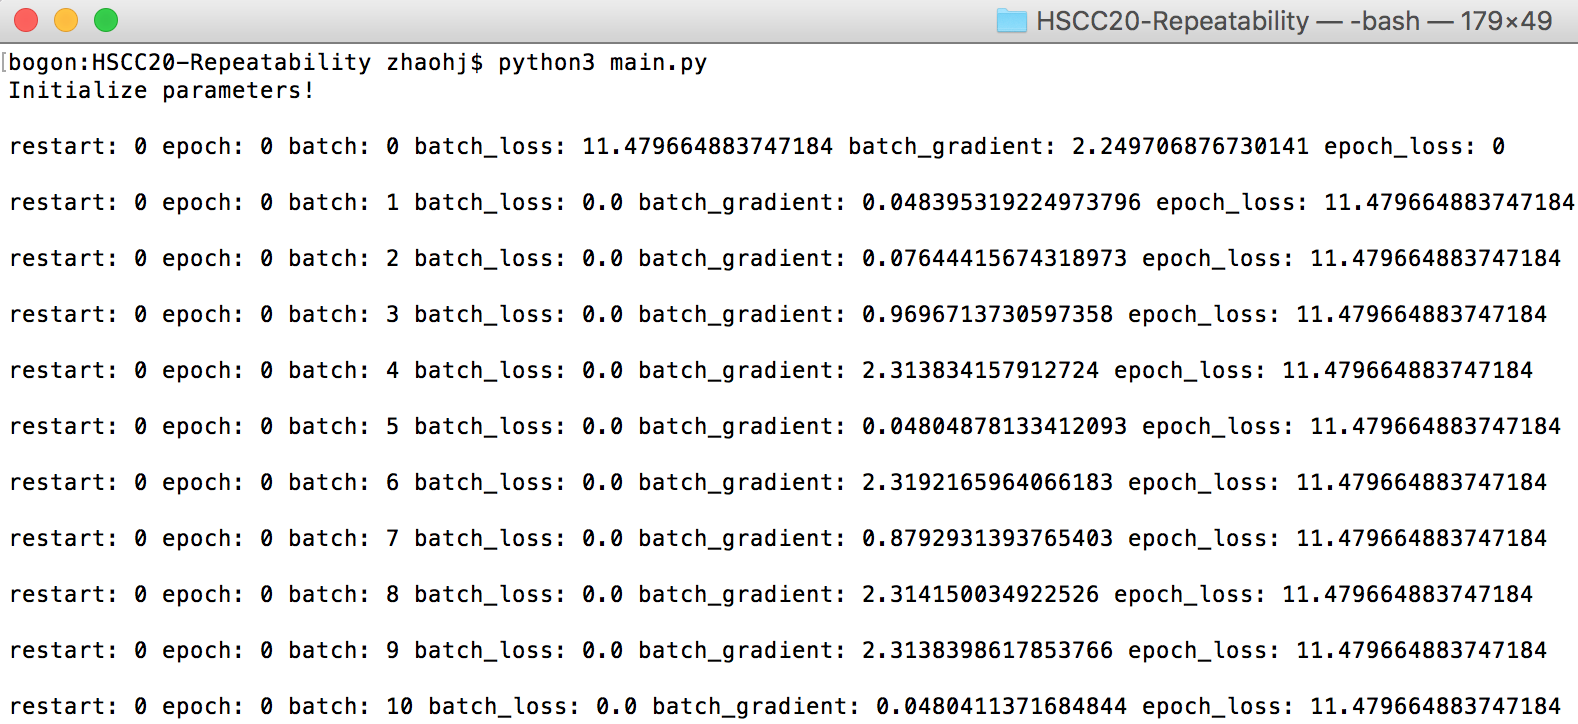
\includegraphics[width=\textwidth]{./fig/training-process}
    \caption{The training process showing the number of restarts, epochs, batches, current gradient, and the current loss} \label{fig:train-process}
\end{figure}

\section{Sample Inputs}
Here we explain more details about the source files, focusing on \textsf{main.py}, and \textsf{prob.py} and \textsf{superp.py} from the sub-folder
{\color{blue}\textsf{eg1\_prajna\_original}} of Example~1. You may skip this and go directly to the next
section for repeatability evaluation, but going through the core codes quickly may enable modifications or extensions of
the reported case studies in our paper.

\subsection{\textsf{main.py}}
Line 
\inputpython{../main.py}{20}{20}
is to build a NN model, the number of layers, neurons, and the type of activation functions of which are specified in \textsf{superp.ty};
Lines
\inputpython{../main.py}{27}{29}
is to generate batches of training data and measure the time cost; 
Lines
\inputpython{../main.py}{32}{34}
are to train the NN model on the generated training data and measure the time cost;
Lines
\inputpython{../main.py}{36}{37}
are to output the measured time costs; Lines
\inputpython{../main.py}{9}{9}
and
\inputpython{../main.py}{44}{44}
are for visualization of the generated barrier certificates, which should be \emph{commented} if you
failed to install the required graphics packages successfully.

\subsection{\textsf{prob.py}}
Line
\inputpython{../cases/eg1_prajna_original/prob.py}{15}{15}
is to set the dimension of the considered system; Lines
\inputpython{../cases/eg1_prajna_original/prob.py}{21}{24}
are to set the interval ranges and the real shape of the initial set, where 1 denotes (super-)rectangle and 
2 denotes circle or sphere; Lines
\inputpython{../cases/eg1_prajna_original/prob.py}{30}{33}
and lines
\inputpython{../cases/eg1_prajna_original/prob.py}{39}{42}
are to set the interval ranges and shapes for the unsafe region and the domain of the system, respectively;
Line 
\inputpython{../cases/eg1_prajna_original/prob.py}{49}{52}
is to set the inequality constraint representing the circle region of the initial set; Lines
\inputpython{../cases/eg1_prajna_original/prob.py}{55}{55}
and 
\inputpython{../cases/eg1_prajna_original/prob.py}{59}{59}
are defining the inequality constraints representing the unsafe and domain areas, respectively;
Lines
\inputpython{../cases/eg1_prajna_original/prob.py}{67}{81}
are defining the continuous dynamics of the considered system, thus finishing the formulation of the
safety verification problem in Example~1.

\subsection{\textsf{superp.py}}

\subsection{User-defined inputs}



% \begin{python}
%     if i==0:
%         abc
%     else:
%         def
% \end{python}
% python3: --version \pyth{__init__}

\section{Repeatability Evaluation}

5 cases, figures, tables

\subsection{Tables}

\begin{itemize}
    \item What elements of the paper are included in the REP (e.g.: specific figures, tables, etc.).
    \item Instructions for installing and running the software and extracting the corresponding results. 
\end{itemize}

\subsection{Figures}

\subsection{Fine-Tuning Figure and Table}

\bibliographystyle{splncs04}
\bibliography{instruction}

% \begin{thebibliography}{8}
% \bibitem{ref_article1}
% Author, F.: Article title. Journal \textbf{2}(5), 99--110 (2016)
% \end{thebibliography}

\end{document}
